\newgeometry{left=1in, right=1in, top=1in, bottom=1.2in}

\chapter{Introduction}
\section{Project Overview}
Credit card fraud detection is a high-impact classification problem in which the goal is to distinguish genuine transactions from fraudulent ones using historical payment data. The difficulty of this task comes from the extreme class imbalance in real-world datasets, where fraudulent cases are rare compared with legitimate transactions. In this project, a supervised machine learning workflow was developed and evaluated on the Kaggle credit card fraud dataset to identify suspicious transactions while maintaining a strong balance between precision and recall.

The dataset contains 284,807 transactions, of which only 492 are fraudulent, making the positive class extremely scarce. This imbalance makes the problem particularly relevant for practical fraud detection systems, where false negatives can be costly and false positives can create unnecessary customer friction. The study therefore focuses not only on predictive accuracy but also on how well the models detect fraud cases without overwhelming the system with incorrect alerts.

\section{Objectives}
The principal objectives of this project were to:
\begin{itemize}
  \item build a reliable fraud detection pipeline using supervised classification models;
  \item compare multiple algorithms under the same evaluation framework;
  \item assess the effect of class imbalance on model behaviour; and
  \item document the workflow, findings, and limitations in a structured report.
\end{itemize}

\chapter{Dataset and Methodology}
\section{Dataset Description}
The dataset used in this study contains transaction-level information obtained from a real-world credit card fraud setting. It includes 30 input variables, where most of the features are anonymised numeric components derived from principal component analysis, along with the transaction time and amount. The target variable, \textit{Class}, indicates whether a transaction is legitimate (0) or fraudulent (1).

A preliminary inspection confirmed that the dataset is complete, with no missing values, and that the class distribution is heavily imbalanced. The prevalence of fraud cases is approximately 0.17\%, which is a typical pattern in fraud detection applications and a key challenge for model training and evaluation.

\section{Experimental Design}
The experimental workflow followed a standard supervised learning structure:
\begin{enumerate}
  \item load and inspect the dataset;
  \item examine the distribution of the target and transaction characteristics;
  \item split the data into training and test sets using a stratified 80/20 ratio;
  \item train several classifiers using the same data partitions; and
  \item evaluate the models using classification metrics that are appropriate for imbalanced data.
\end{enumerate}

Because accuracy alone can be misleading when one class is extremely rare, the analysis emphasised precision, recall, F1-score, and ROC-AUC. These metrics are more informative in fraud detection because they reflect how well the model identifies fraudulent transactions while controlling the volume of false alarms.

\chapter{Exploratory Data Analysis}
\section{Class Distribution and Data Characteristics}
A visual inspection of the dataset confirms the severity of the class imbalance. Legitimate transactions dominate the sample, while fraudulent transactions are sparse and concentrated in a very small fraction of the observations. This structure strongly influences model behaviour and explains why simple accuracy-based interpretation can be deceptive in this setting.

\begin{figure}[H]
  \centering
  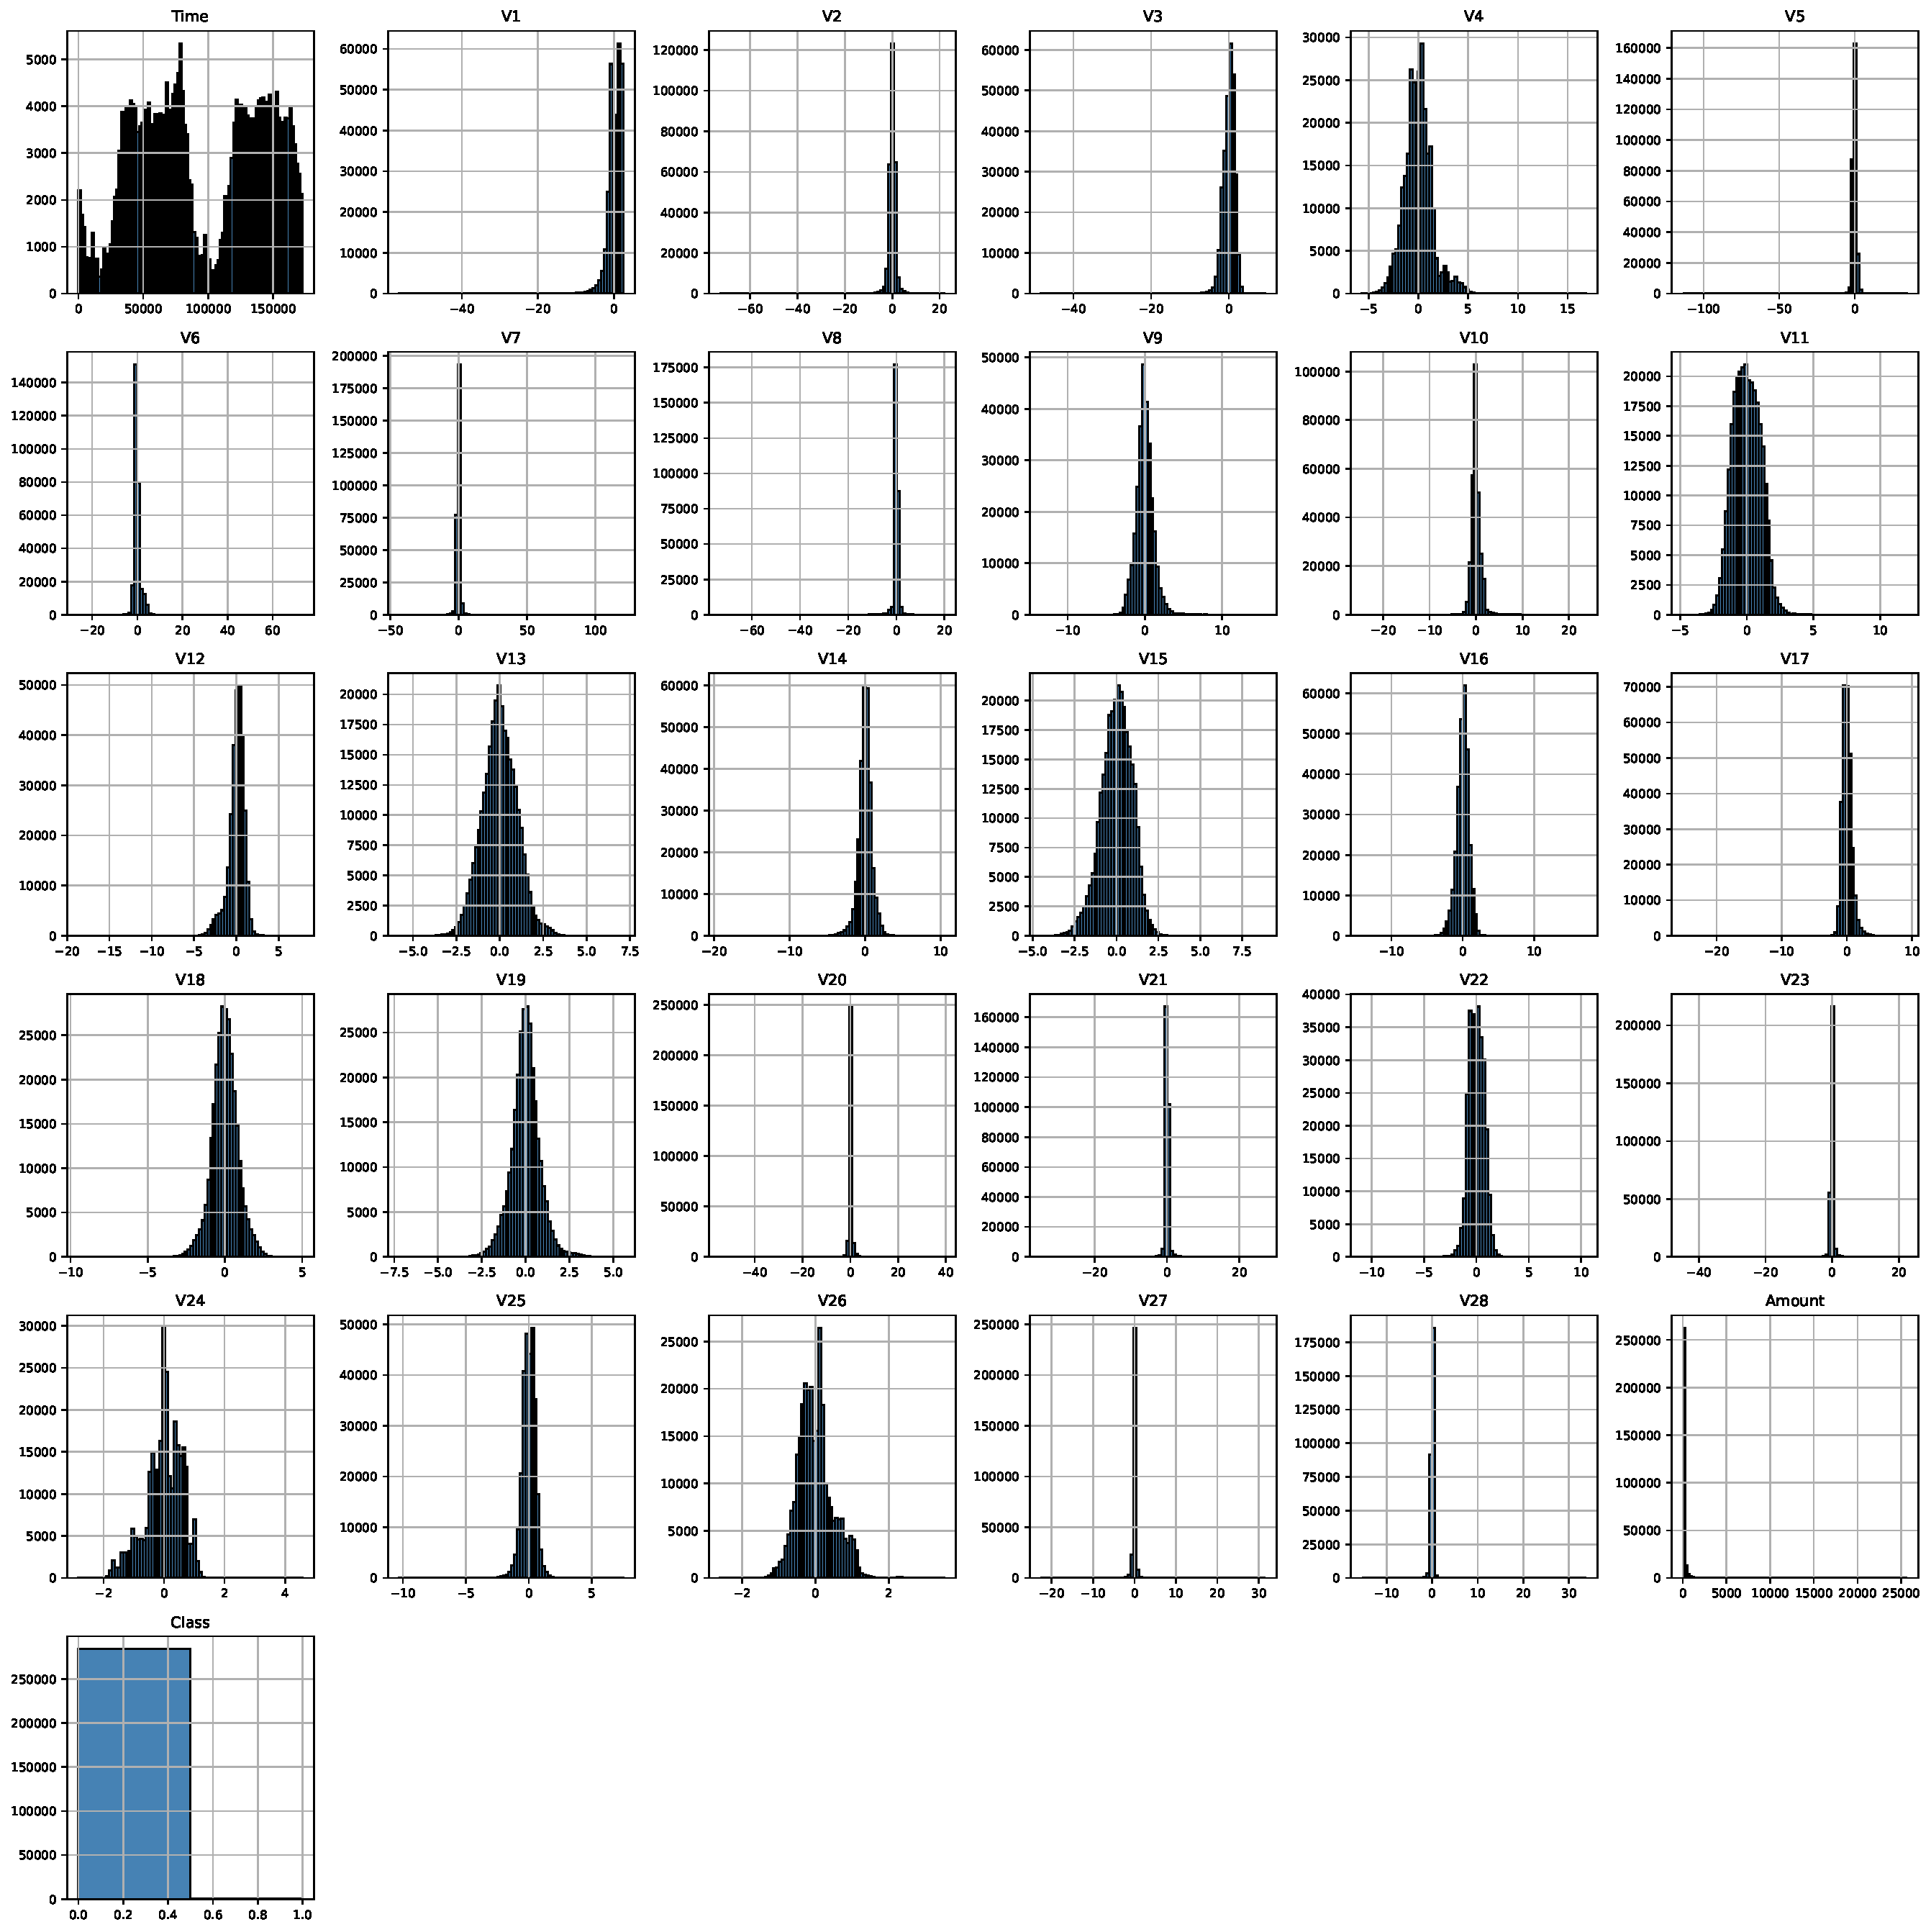
\includegraphics[width=0.95\textwidth]{../figures/creditcard_distribution.pdf}
  \caption{Distribution of the fraud and non-fraud classes in the credit card dataset.}
\end{figure}

\section{Feature Relationships and Correlation Patterns}
The exploratory analysis also examined the relationships among the transformed features and the target variable. The anonymised PCA components present a complex structure, and their interactions are not obvious from simple univariate inspection. Nevertheless, the correlation analysis reveals that several features carry useful signal for separating fraudulent from legitimate transactions, even though the relationships are not always direct or linear.

\begin{figure}[H]
  \centering
  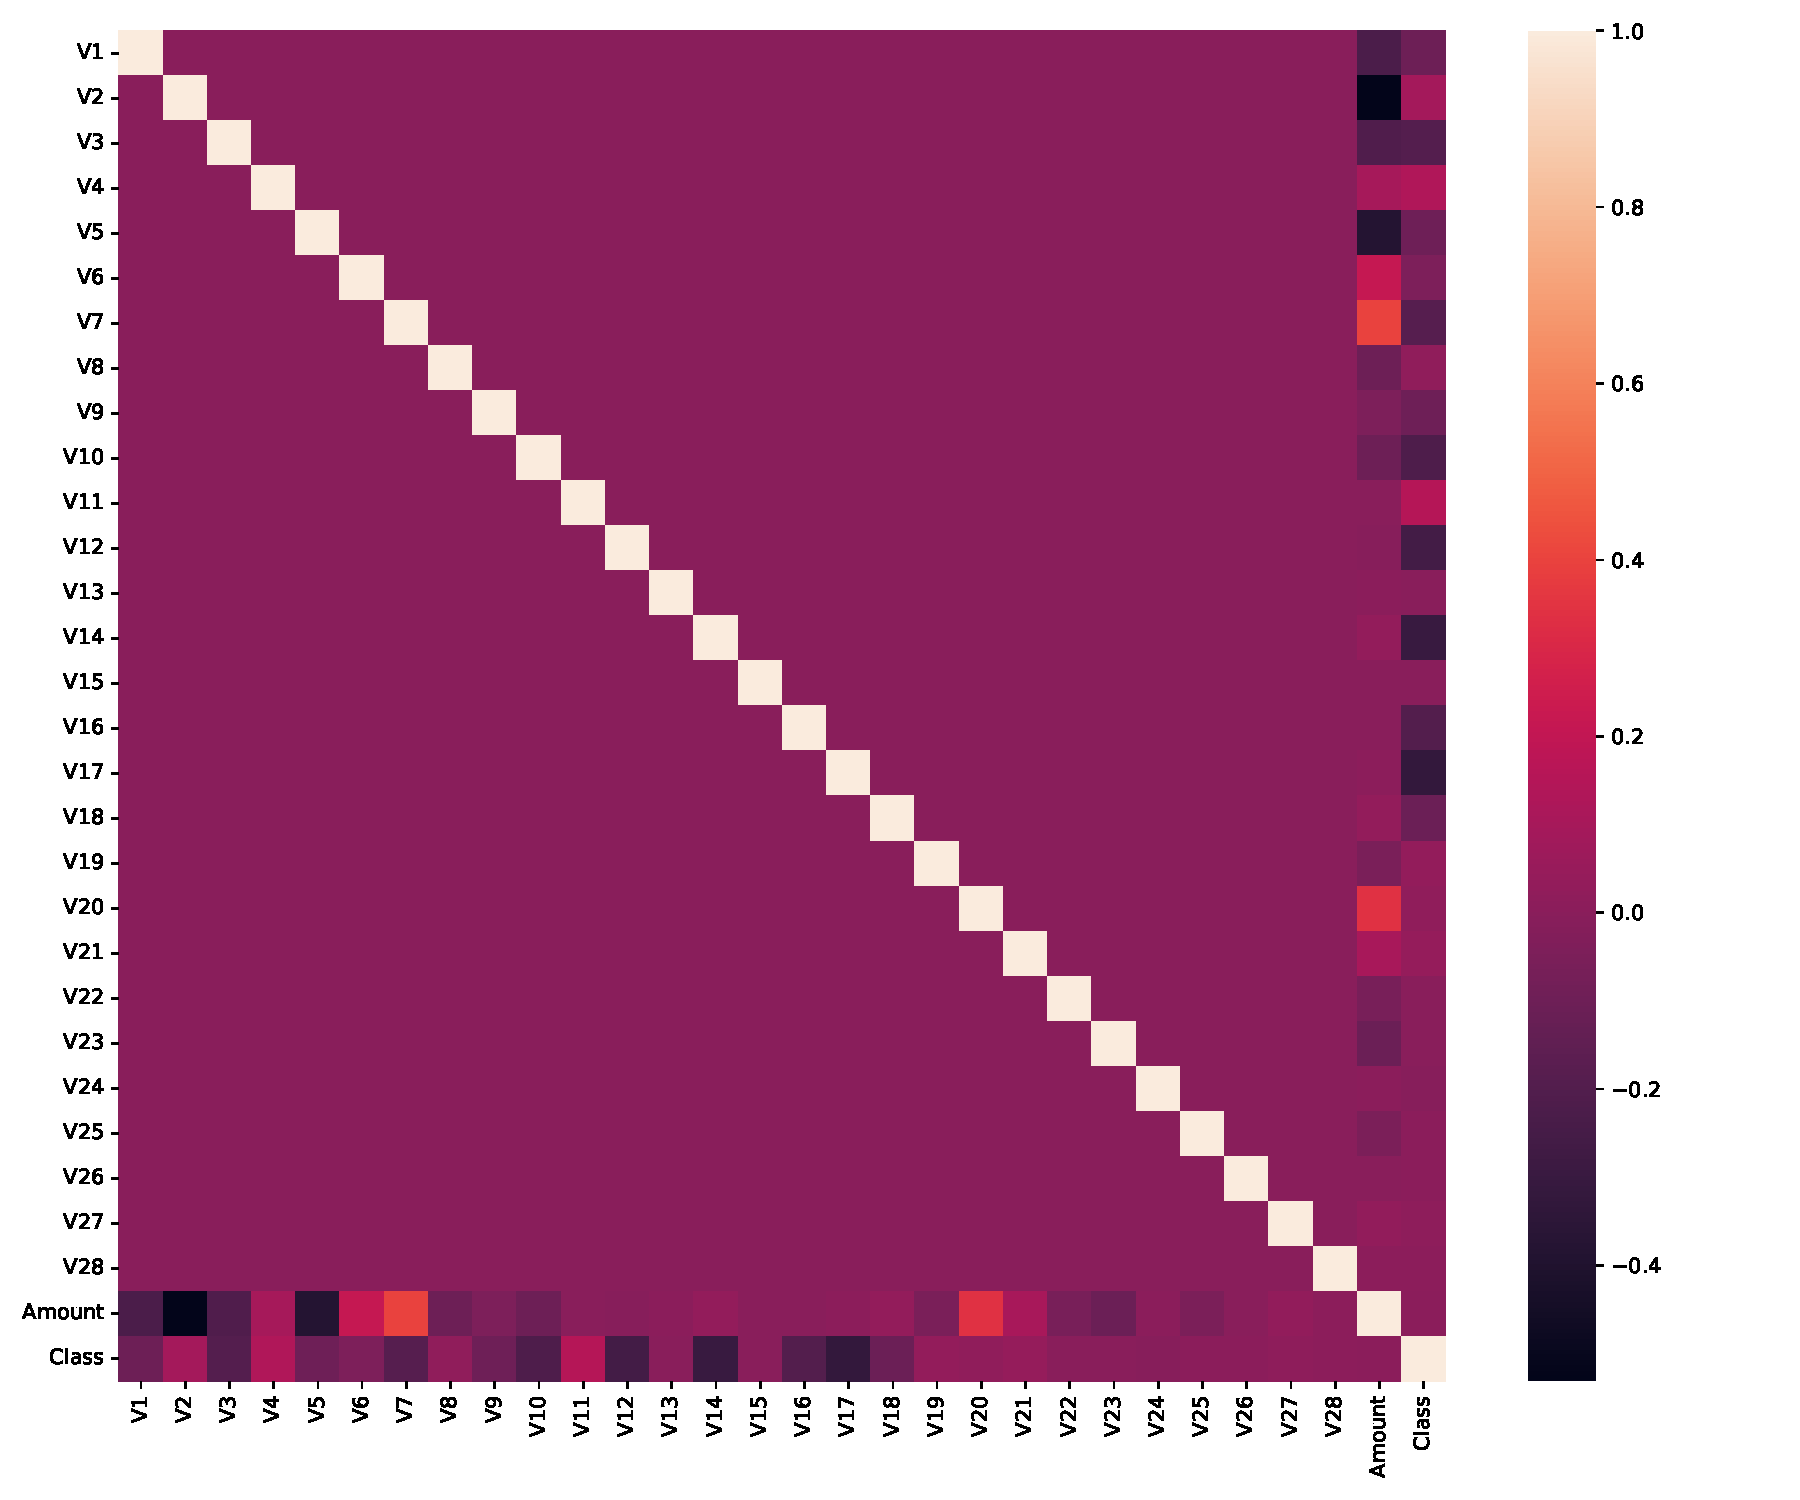
\includegraphics[width=0.95\textwidth]{../figures/variable_correlations.pdf}
  \caption{Correlation structure among the numerical variables used in the fraud detection models.}
\end{figure}

This exploratory stage supports the use of flexible classifiers that can capture non-linear decision boundaries and detect subtle deviations associated with fraudulent behaviour.

\chapter{Model Development and Evaluation}
\section{Models Compared}
Several classification models were trained and compared to identify the most suitable approach for fraud detection. The models included:
\begin{itemize}
  \item Logistic Regression;
  \item Linear Support Vector Machine;
  \item Random Forest Classifier;
  \item Gradient Boosting Classifier; and
  \item a Stacking Classifier combining tree-based learners with a logistic regression final estimator.
\end{itemize}

The evaluation focused on metrics that are meaningful under imbalance conditions. In particular, recall was treated as essential because it measures the proportion of actual fraud cases correctly detected, while precision indicates how reliable the positive predictions are. The F1-score was used as a balanced summary of both measures.

\begin{table}[H]
  \centering
  \caption{Performance comparison of the evaluated classification models.}
  \begin{tabular}{lcccc}
    \toprule
    Model & Accuracy & Precision & Recall & F1-score \\
    \midrule
    Logistic Regression & 0.9755 & 0.0610 & 0.9184 & 0.1144 \\
    Linear SVM & 1.0000 & 0.80 & 0.58 & 0.67 \\
    Random Forest & 1.0000 & 0.88 & 0.80 & 0.83 \\
    Gradient Boosting & 1.0000 & 0.94 & 0.74 & 0.83 \\
    Stacking Classifier & 1.0000 & 0.95 & 0.71 & 0.81 \\
    \bottomrule
  \end{tabular}
\end{table}

The table shows an important pattern: the best-performing models are those that improve precision substantially while retaining strong recall. Logistic regression, although highly sensitive to fraud cases, produces a large number of false positives, which makes it less useful in a practical fraud monitoring system. By contrast, the ensemble methods provide a more balanced and operationally useful trade-off.

\section{Diagnostic Analysis}
The diagnostic plots generated for the main classifiers provide further evidence that the tree-based models are better suited to this problem than the linear baseline. The visualisations show more stable decision boundaries and better separation between the fraud and non-fraud classes when non-linear structures are allowed.

\begin{figure}[H]
  \centering
  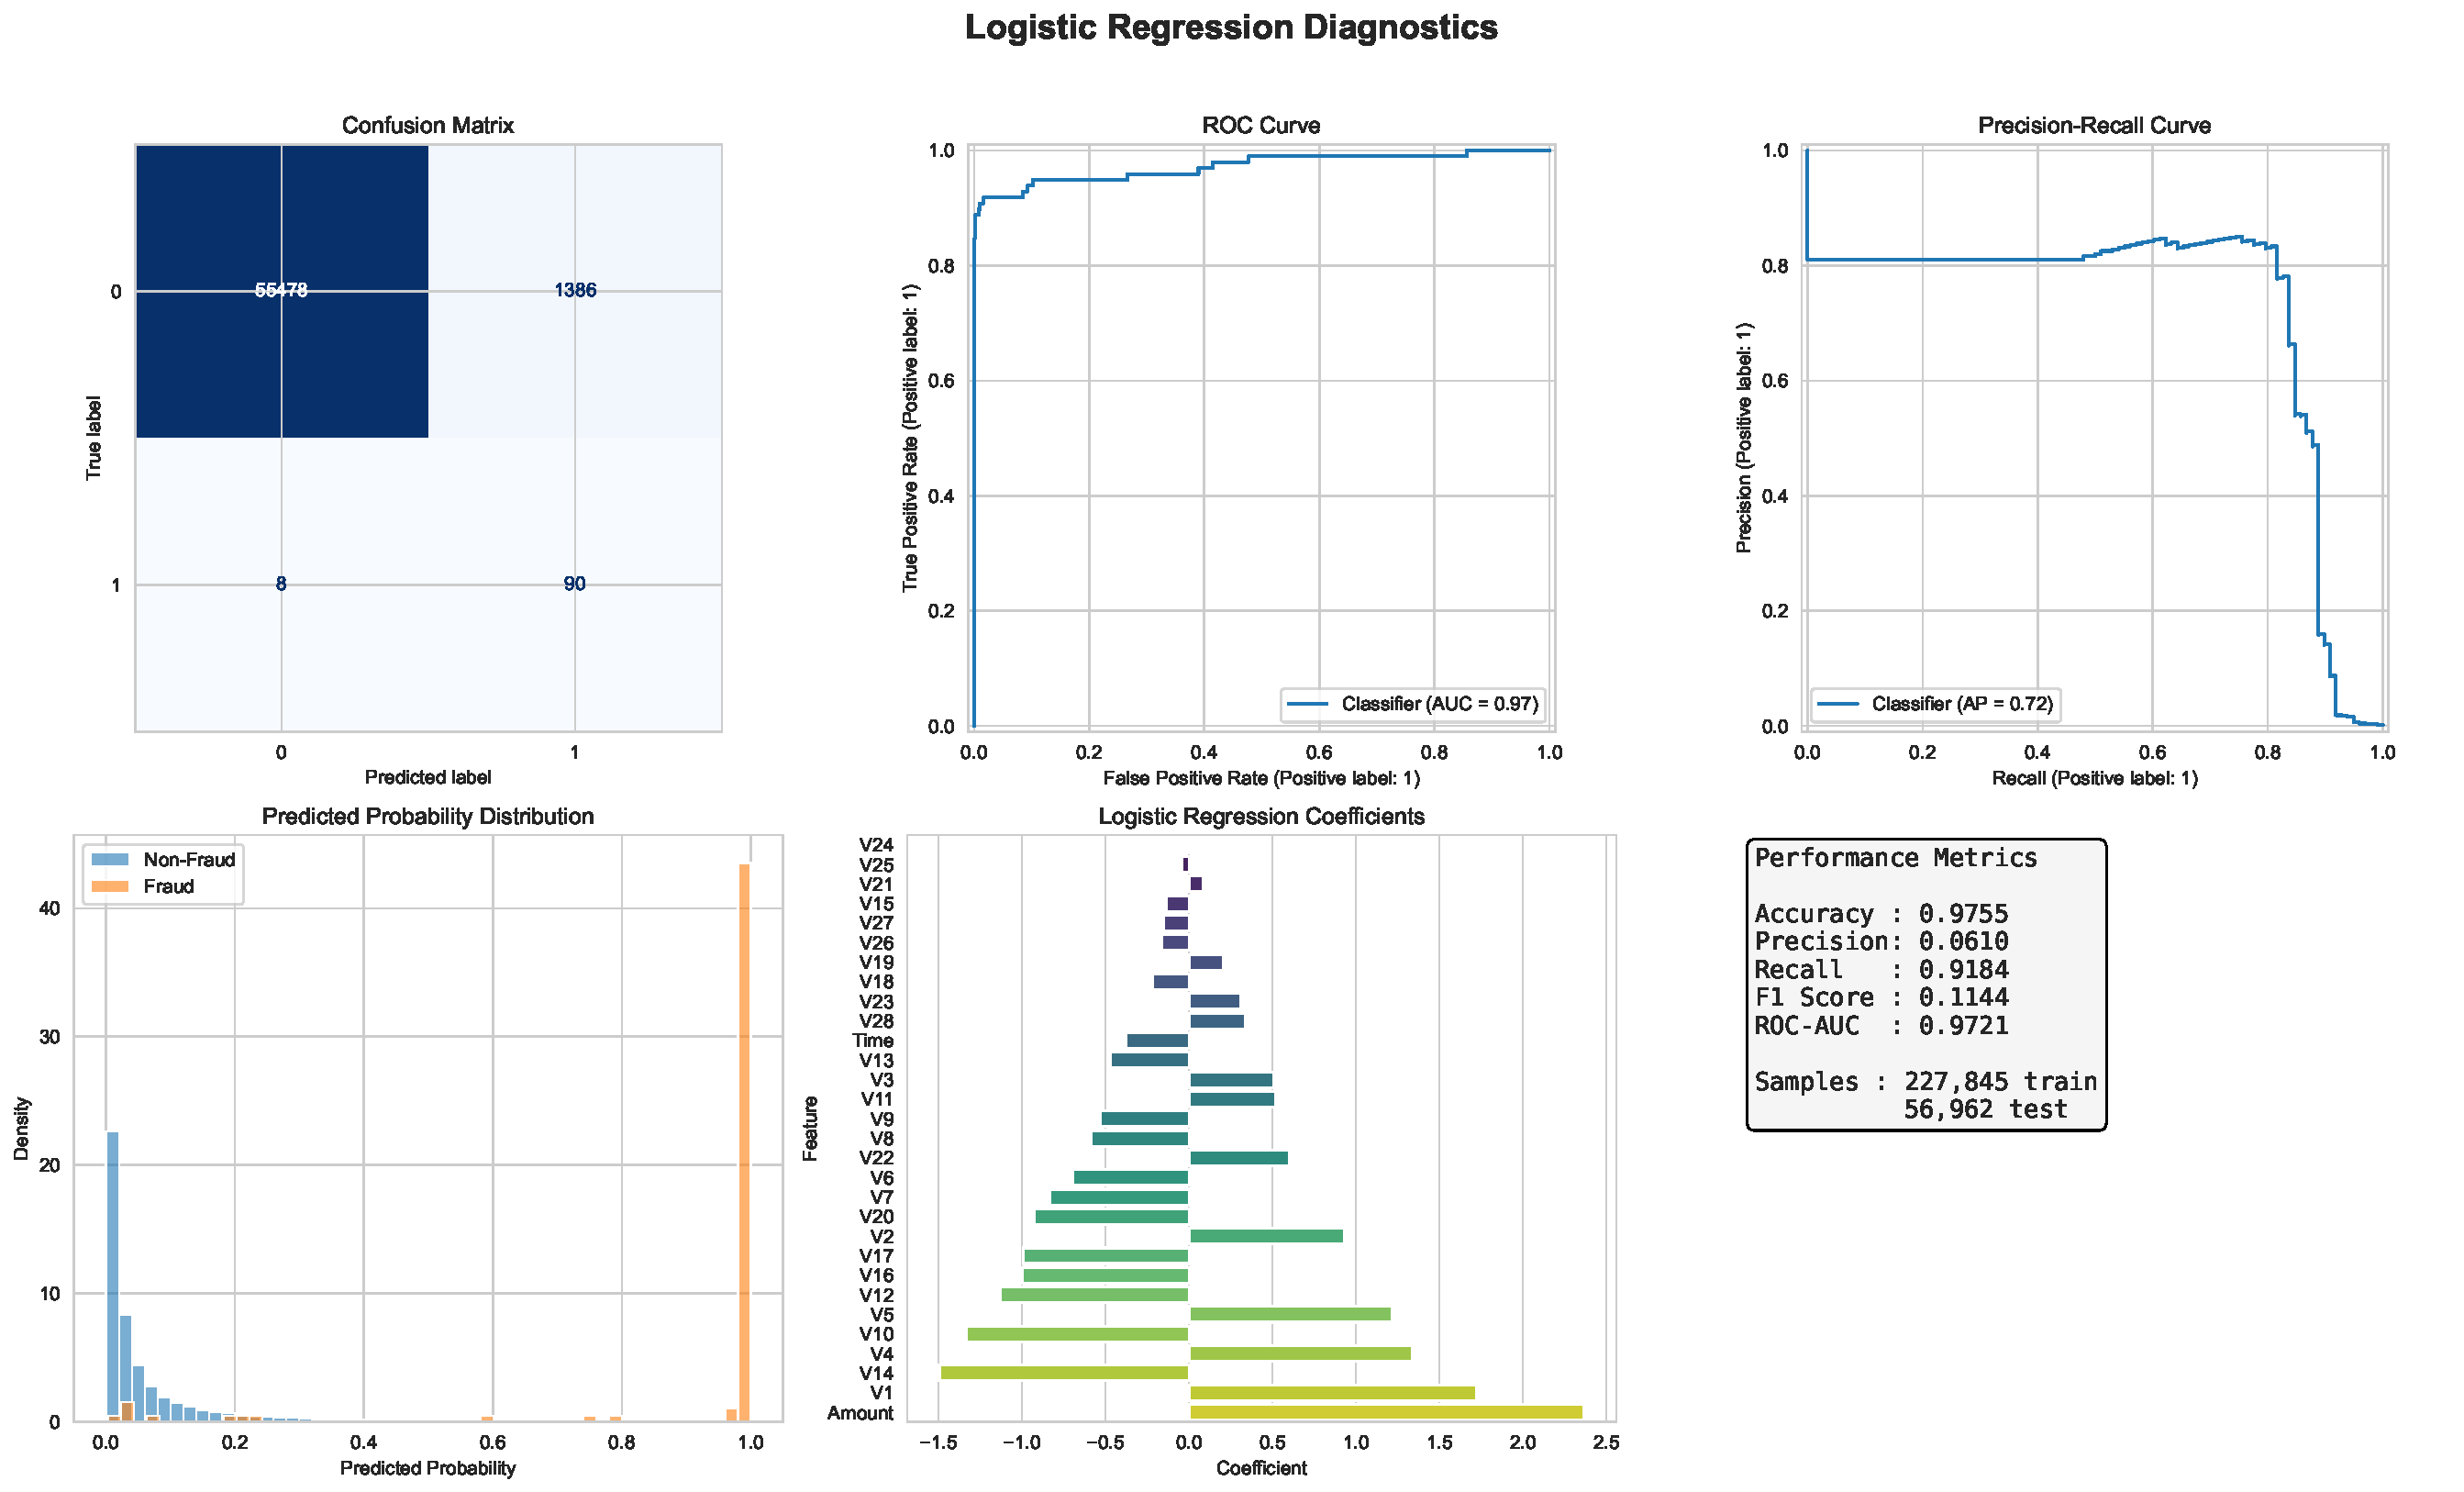
\includegraphics[width=0.95\textwidth]{../figures/logistic_regression_diagnostics.pdf}
  \caption{Diagnostic evaluation of the logistic regression classifier.}
\end{figure}

\begin{figure}[H]
  \centering
  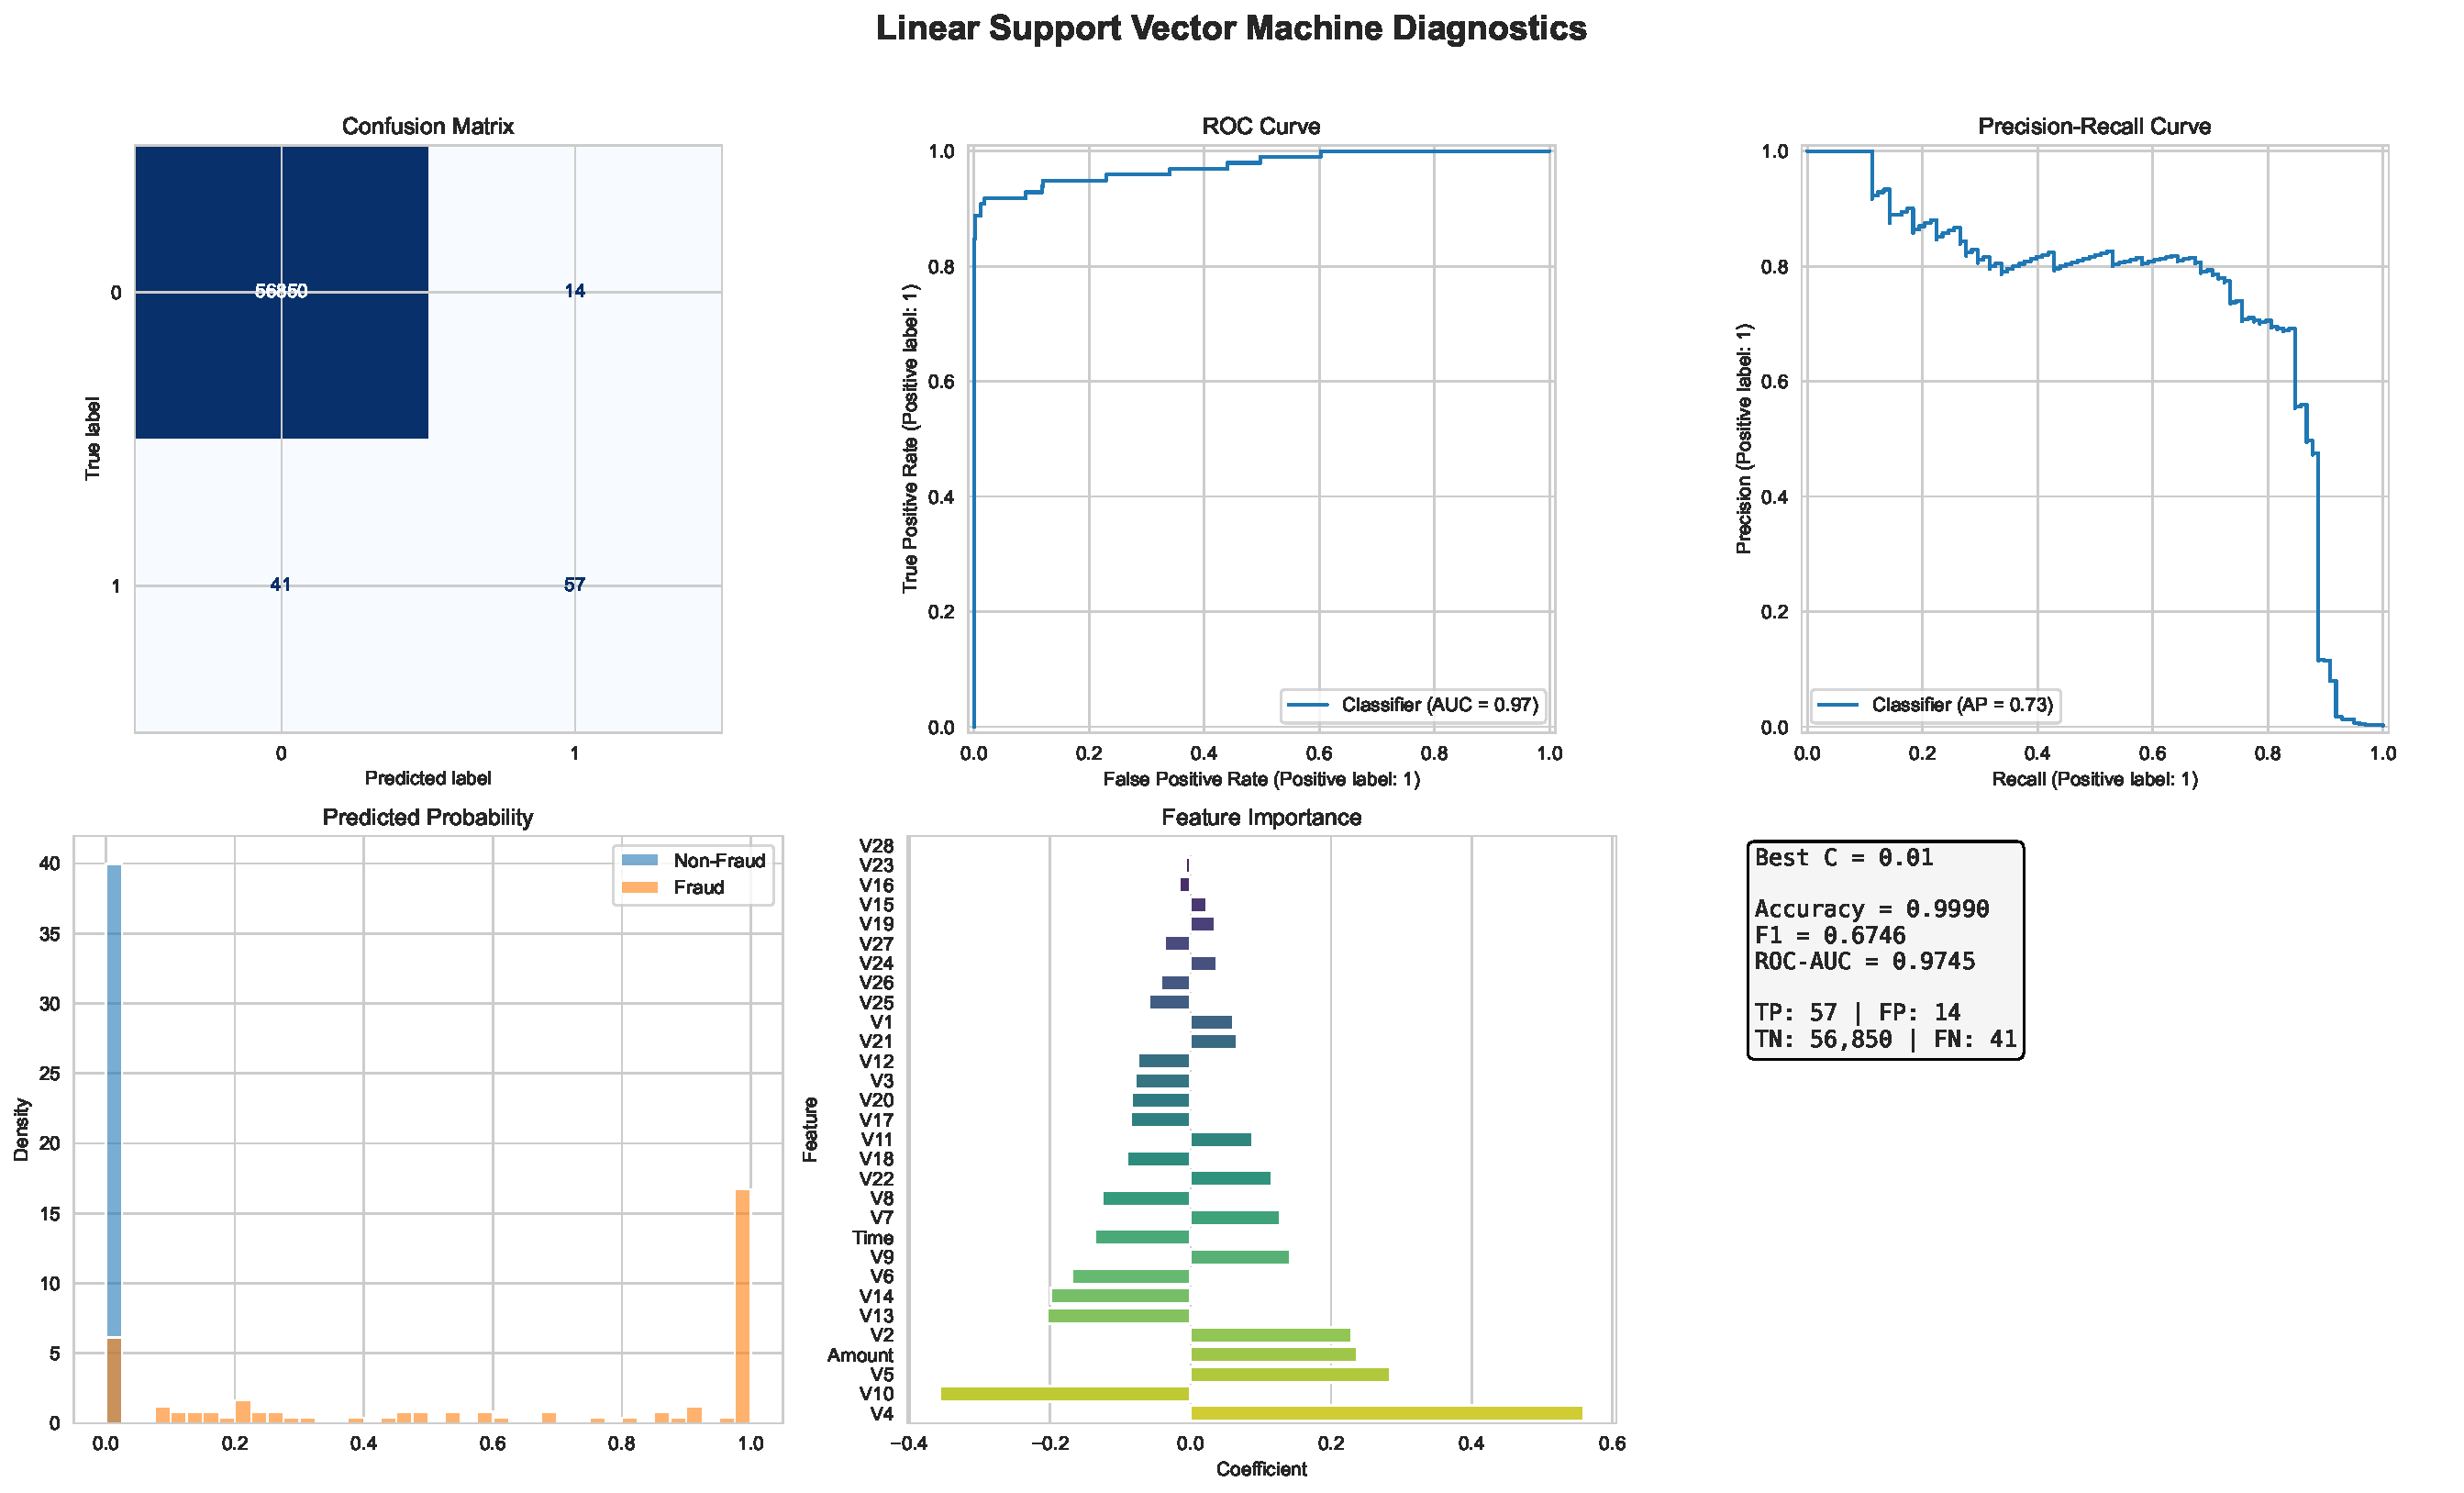
\includegraphics[width=0.95\textwidth]{../figures/linear_svm_diagnostics.pdf}
  \caption{Diagnostic evaluation of the linear SVM classifier.}
\end{figure}

\begin{figure}[H]
  \centering
  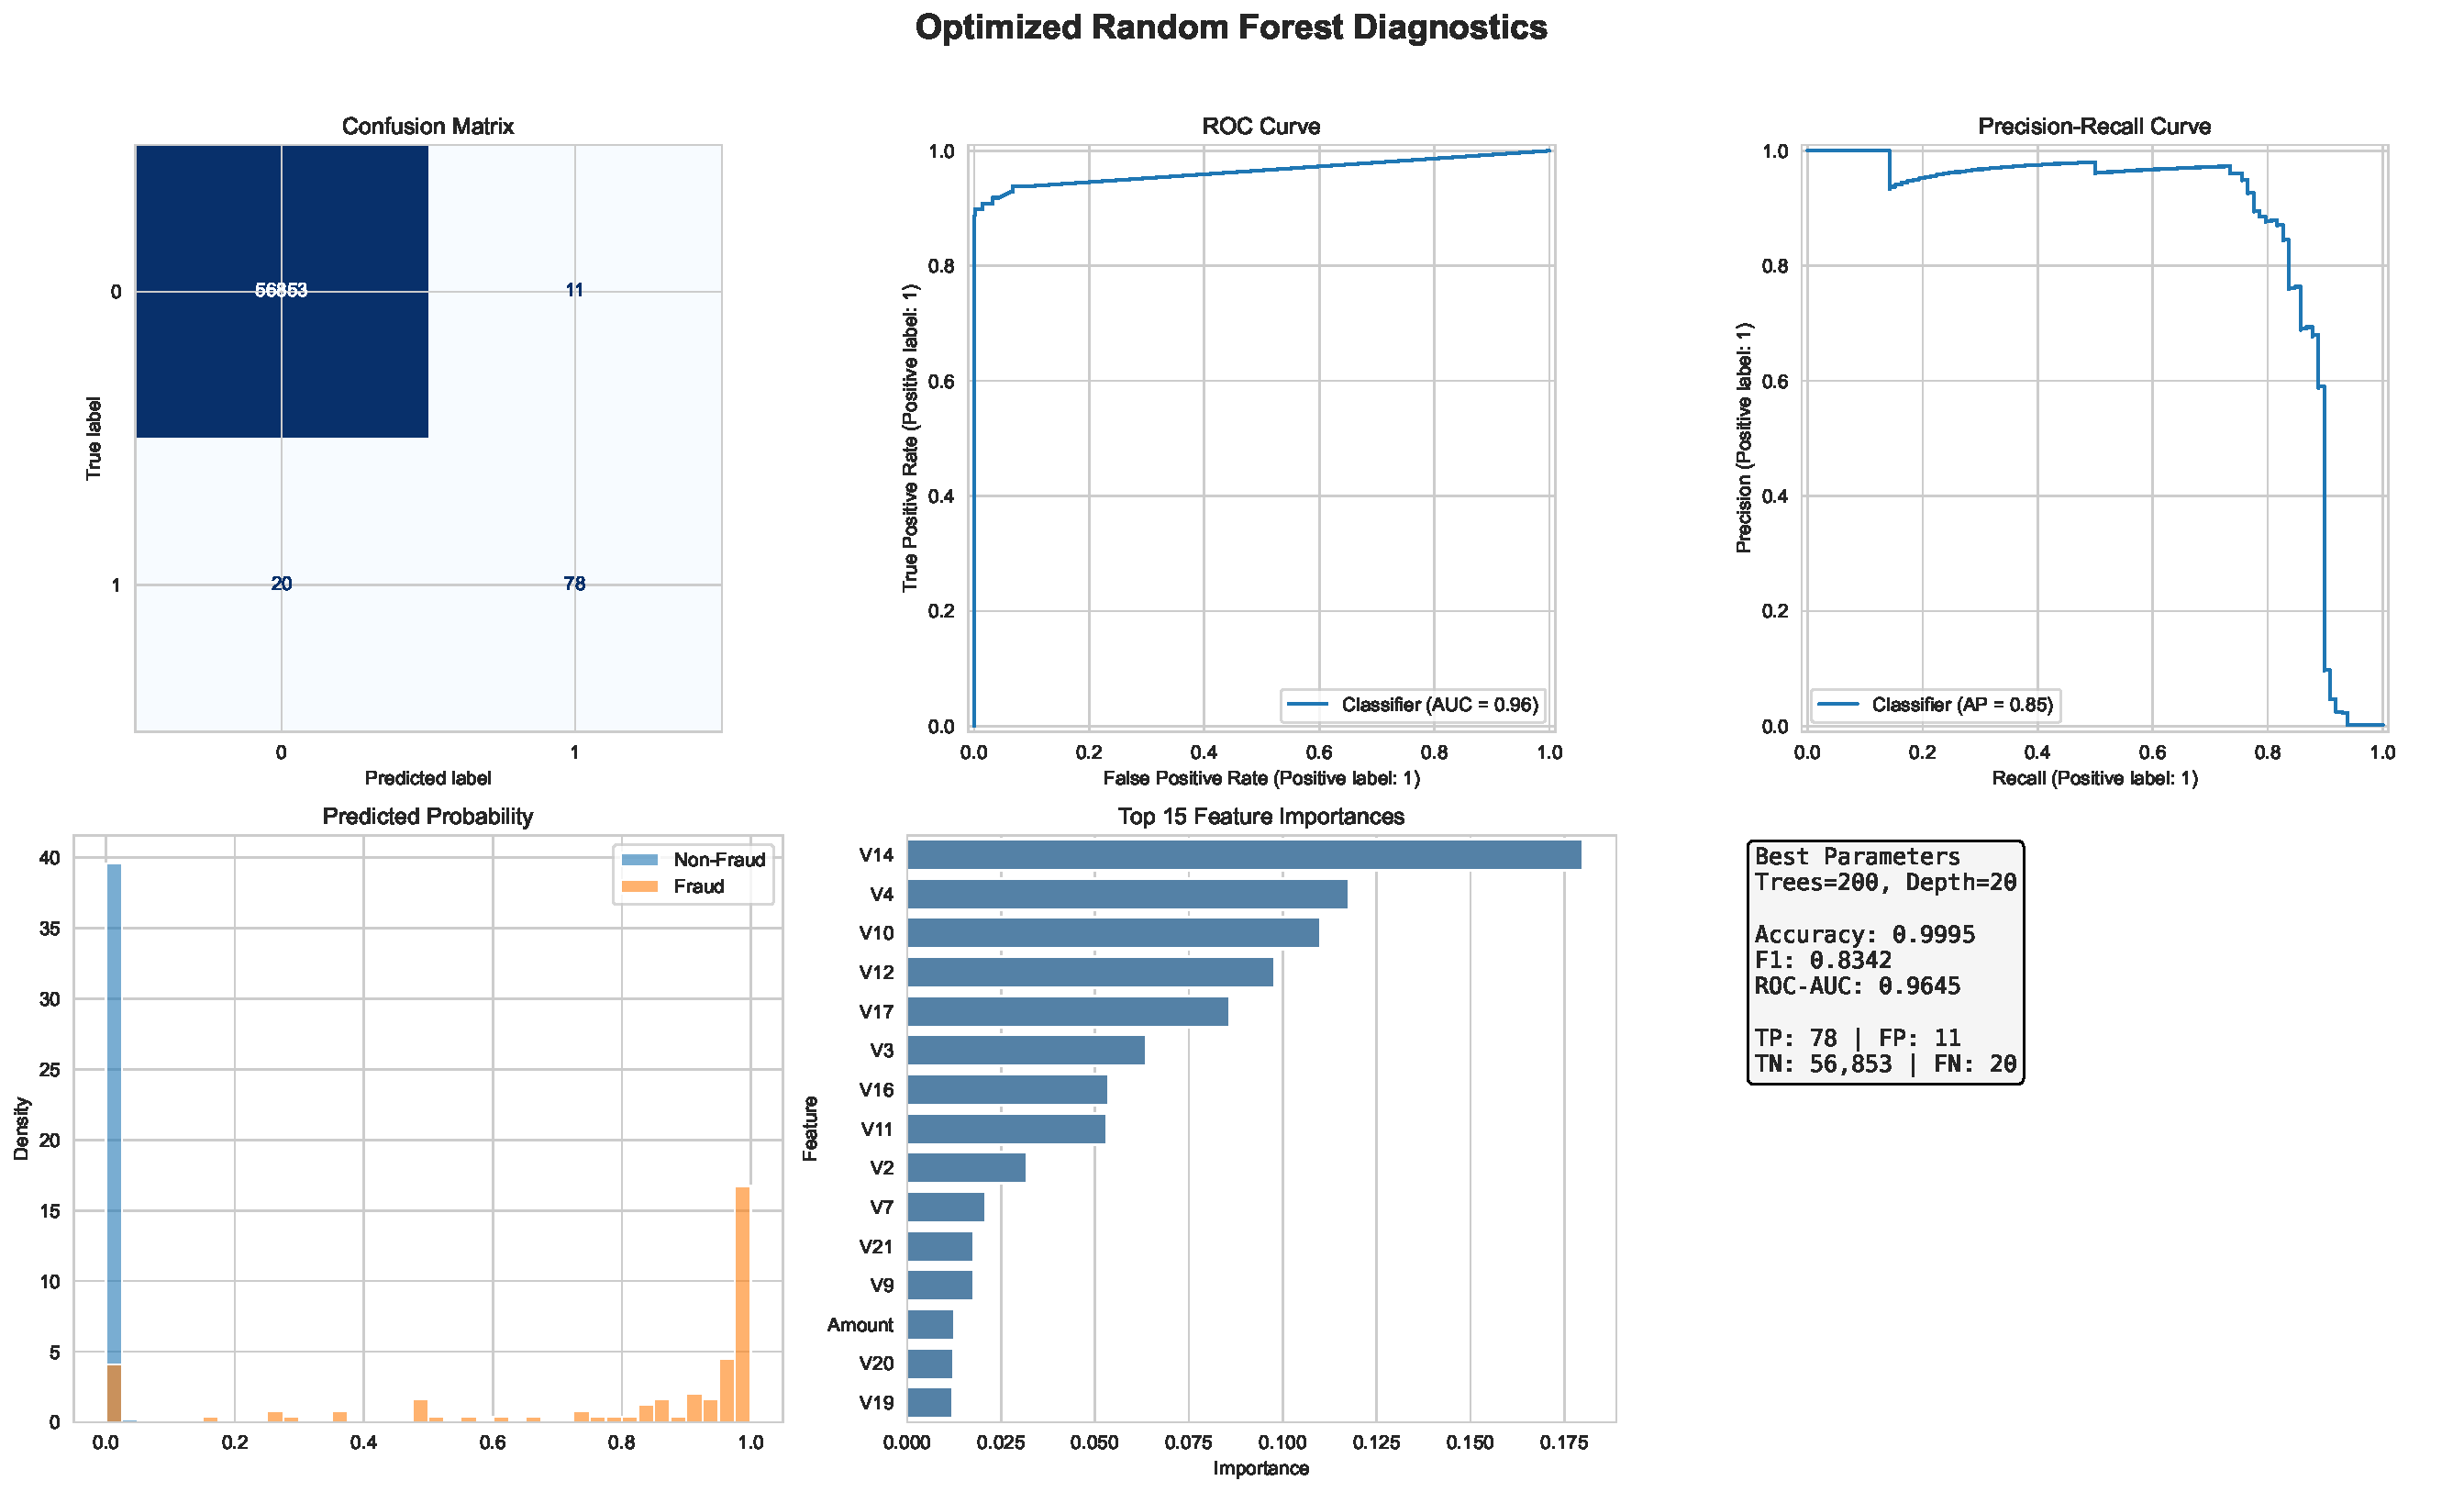
\includegraphics[width=0.95\textwidth]{../figures/rf_diagnostics_optimized.pdf}
  \caption{Diagnostic evaluation of the optimized random forest classifier.}
\end{figure}

\begin{figure}[H]
  \centering
  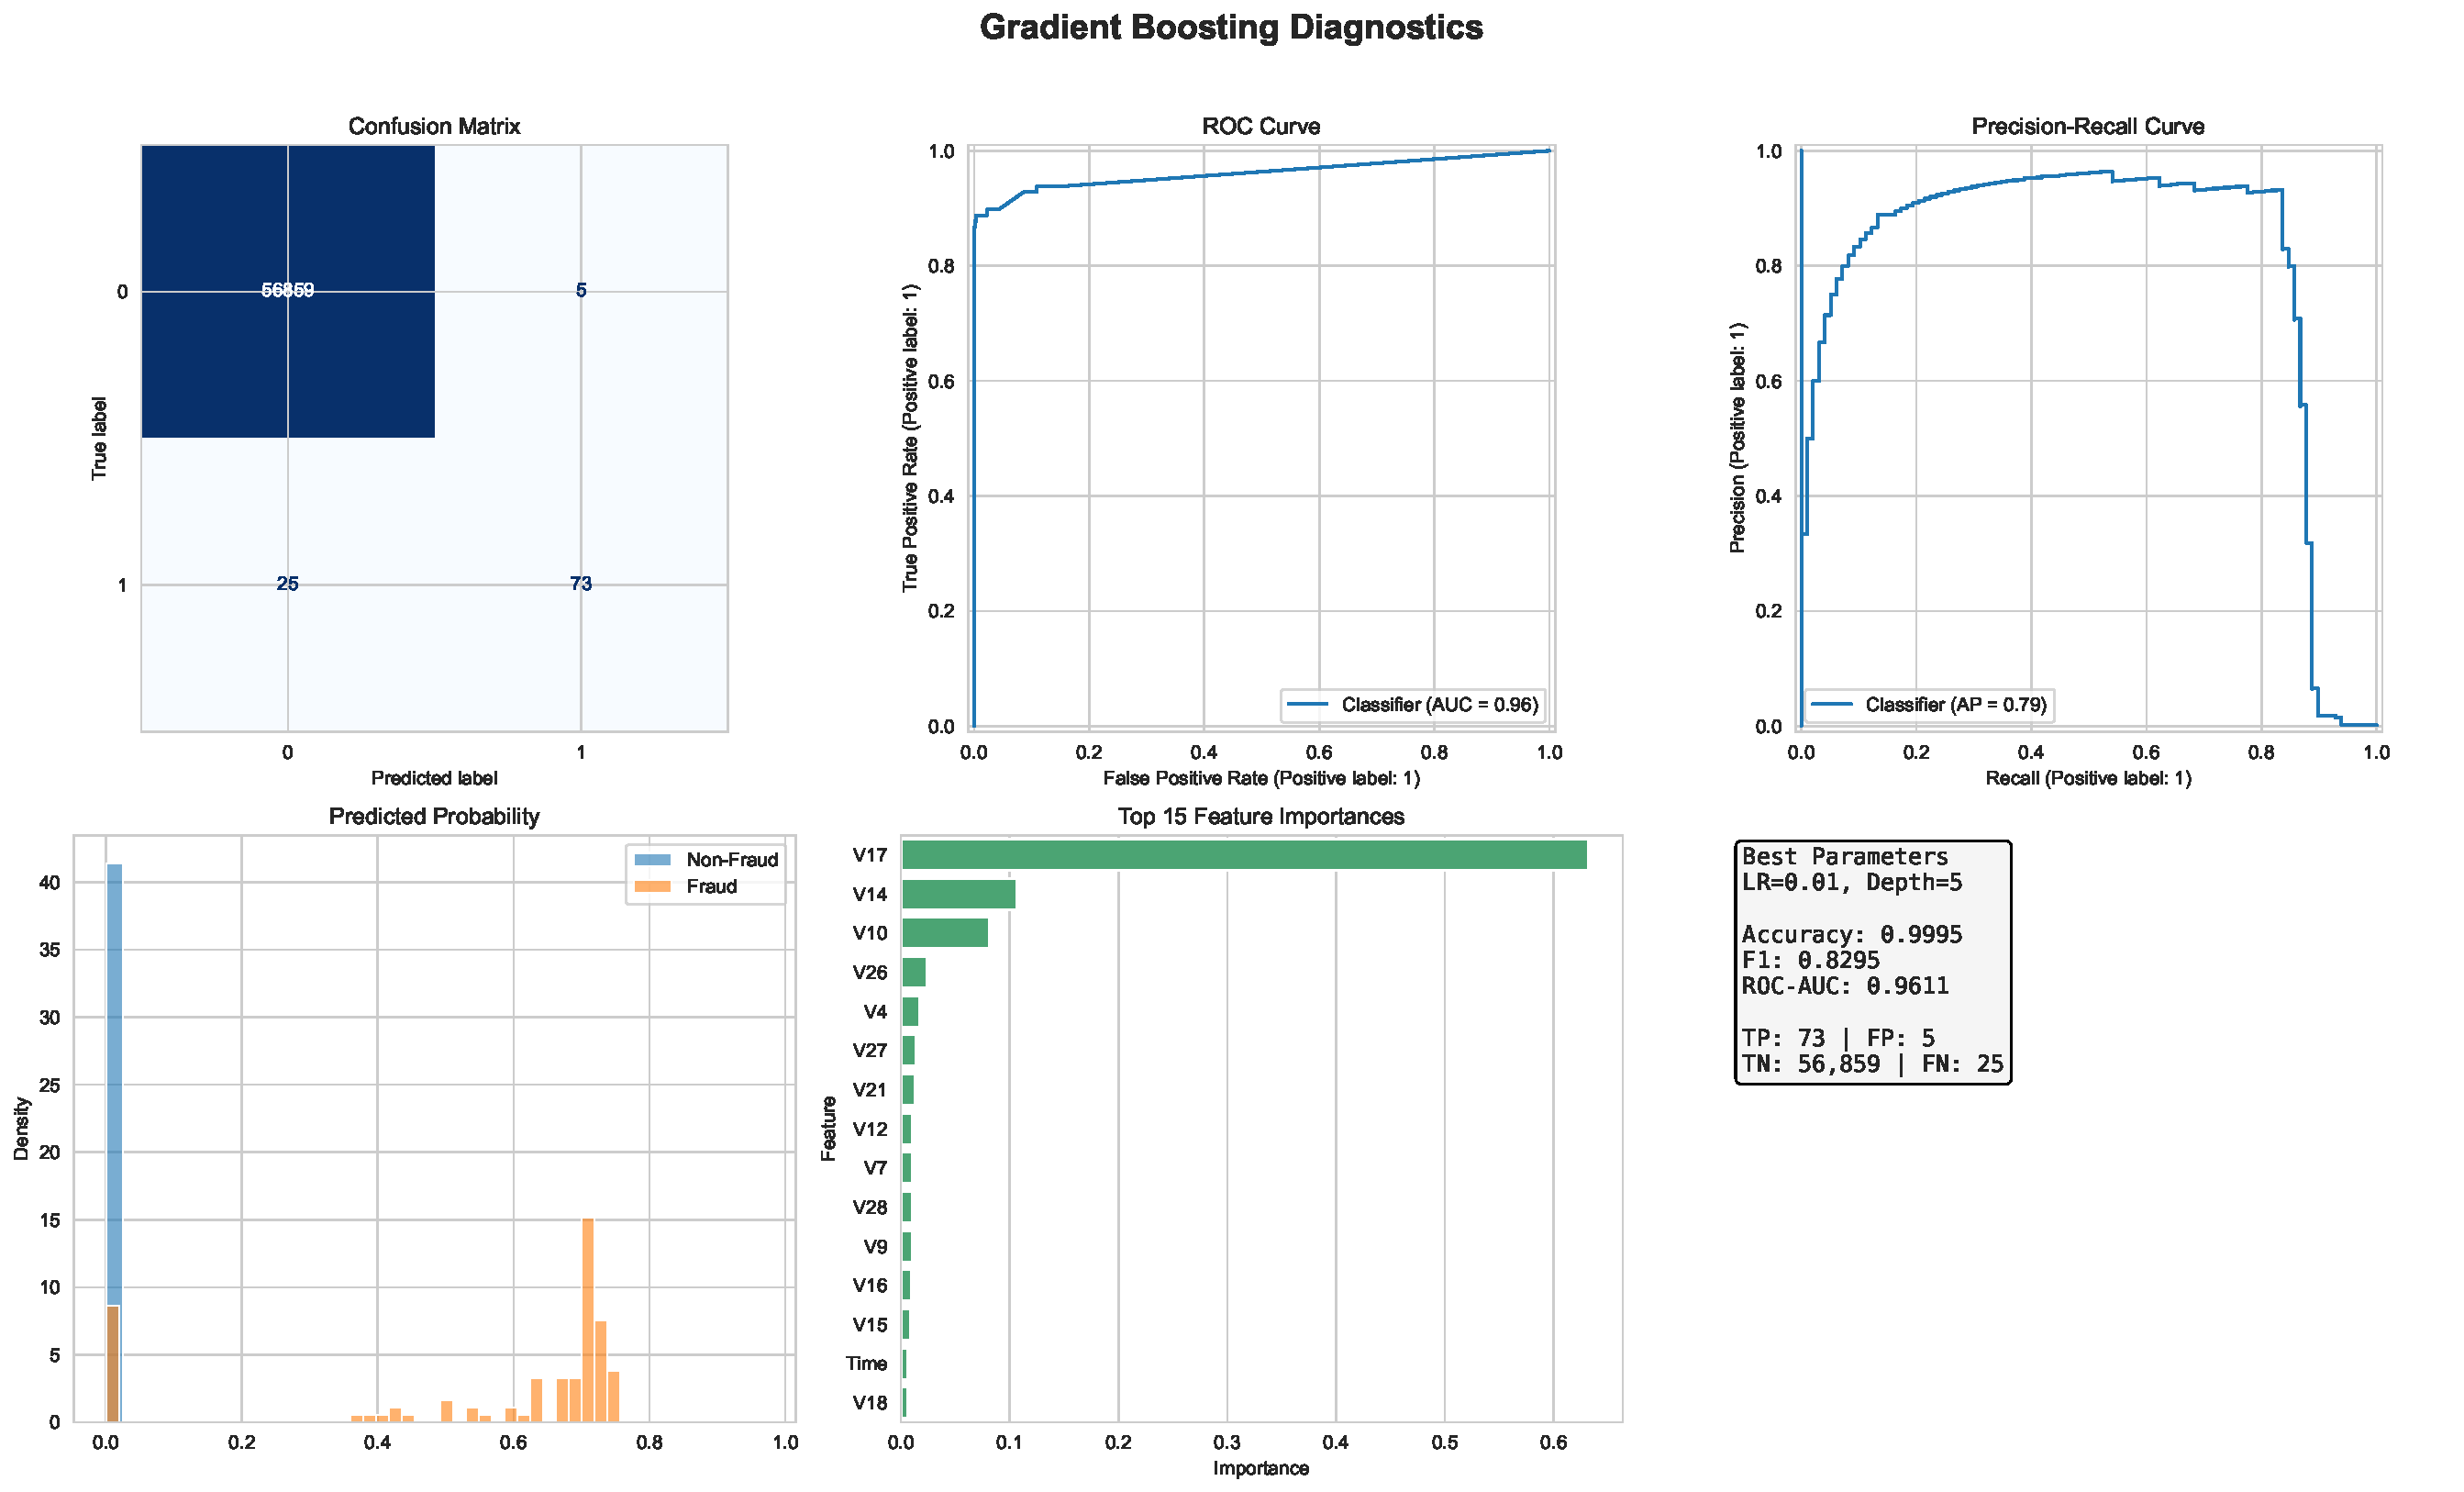
\includegraphics[width=0.95\textwidth]{../figures/gbc_diagnostics.pdf}
  \caption{Diagnostic evaluation of the gradient boosting classifier.}
\end{figure}

\chapter{Discussion}
The most important insight from this project is that fraud detection is not a standard balanced-class classification problem. The strong imbalance means that a model can appear highly accurate while still missing many fraudulent transactions. Consequently, the evaluation must focus on the ability to detect the minority class reliably rather than on raw accuracy alone.

The comparison of models indicates that tree-based ensemble methods offer the most practical performance for this application. Random Forest and Gradient Boosting achieved the highest precision and F1-scores among the tested models, suggesting that they are better at limiting false alarms while still capturing a high share of fraud cases. The Stacking Classifier also performed well, but its improvement over the best single ensemble was modest, which suggests that the additional complexity may not always be justified in this setting.

The linear SVM also showed reasonable performance but was less effective at recovering the minority class than the tree-based methods. Its lower recall indicates that some fraud cases remain undetected, which is a significant concern in real-world fraud prevention systems. In contrast, logistic regression demonstrated very high recall but poor precision, implying that it flagged many legitimate transactions as suspicious.

\chapter{Conclusion}
This project developed and evaluated a supervised machine learning workflow for credit card fraud detection. The study demonstrated that fraud data can be modelled effectively using classification algorithms, but that success depends heavily on choosing evaluation metrics that reflect the imbalance in the data. Among the tested models, the tree-based ensemble classifiers provided the most balanced and reliable results, with Random Forest and Gradient Boosting delivering the strongest overall performance.

Overall, the analysis confirms that machine learning classification can be a valuable tool for fraud detection, particularly when the goal is to detect rare events with high precision and acceptable recall. Future work could explore class-weighting strategies, anomaly detection methods, or more advanced ensemble approaches to further improve the detection of fraudulent transactions while lowering false-positive rates.
